\Chapter{CONVOLUTIONAL NEURAL NETWORK WITH COMMENTS AND SOURCE CODE}\label{sec:Theme3}

% TOTAL = 15 pages

%	./train.py --enable_word_embeddings true --num_epochs 6 --dev_sample_percentage 0.01 --positive_train=$pos --negative_train=$neg
%	
%	Used for the 3-Folds
%
% ./word2vec -train ../../tokenized-concordia-no-comment.txt -output concordia-bin-64.bin -size 100 -window 5 -sample 1e-4 -negative 5 -hs 0 -binary 1 -cbow 1 -iter 3

\section{Convolutional Neural Network}

%1 page

Several machine learners were tested with TEDIOUS, using source code metrics as training features. Results were promising but the approach asked for a lot of preparation work: building the XML representation of the Java code, pattern matching between comments from the dataset and the source code, extracting the source code metrics, extracting the warning raised by static analysis tools and feature preprocessing. These additional steps take time and knowledge of the whole process. Consequently, we wanted to try a novel approach, easier and faster to set up. We decided to test a Convolutional Neural Network (CNN) with Natural Language Processing (NLP) directly on the Java source code of software projects.

The idea of using a CNN was inspired by a paper written by \citet{kim2014convolutional}. He used a CNN for sentence-level classification tasks and showed that you can achieve excellent performance results with little parameter calibration. He tested his model on several benchmarks. Similar work has been pursued concerning sentiment analysis of short texts \citep{dos2014deep}. More specifically, they analyzed Twitter messages and movie reviews, and tried to classify them as being of positive or negative sentiment. Our idea is similar to these studies, we plan to use a CNN to classify comments and/or methods using the source code directly instead of features, linking them to technical debt or not.

Typically, convolutional neural networks were employed for image classification \citep{krizhevsky2012imagenet}, however, as mentioned previously, this type of neural network has been used recently combined with NLP. To describe CNN in further details, we can think of a convolution as a window sliding across a whole matrix, acting as a filter. For images, this matrix contains pixels, for words and sentences, it contains word vectors (word embeddings). In image classification, filters slide over local batches, in NLP, they slide over entire rows since a row is typically a single word embedded into a row matrix of the size of the embedding dimension. To implement a CNN, you just have to add several layers of these convolutions, where each of these layers have a specific task and act as different filters. CNNs are very fast and efficient in terms of representation, which means they give good representations without needing the whole vocabulary of a dataset.

The main purpose of this study was to explain, test and analysis TEDIOUS, our machine learning approach using source code features. The next sections will describe the other approach using a CNN, but at a more general level than for TEDIOUS since we are still at a preliminary stage. Since some steps from Chapter 3 are replicated in our CNN approach, they will be explained rapidly in order to avoid redundancy. However, we still judged interesting to present the initial results of this new promising method.

\section{The Approach}

%1 page

This section will describe the steps followed to design this new approach, a convolutional neural network combined with natural language processing to identify technical debts to self-admit. Additional information will be shared on the characteristics of this machine learner and how it works. Like TEDIOUS, this approach works at method-level since it is granularity at which we are most likely to detect TD \citep{PotdarS14}. In other terms, this approach is able to detect if a technical debt is contained in a method or not.

\begin{figure}[t]
	\centering
	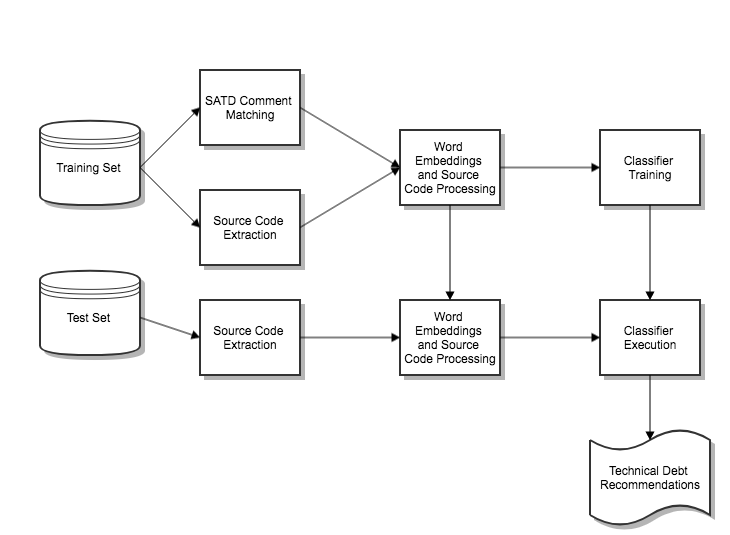
\includegraphics[width=\linewidth]{figs/CNN.png}
	\caption{Proposed approach for recommending SATD with a CNN.}
	\label{fig:CNN}
	\vspace{-4mm}
\end{figure}

As shown in Figure \ref{fig:CNN}, two datasets are required to build our model: the training and test set. The training set contains labeled data, which is source code where SATD are known. The test set contains unlabeled data, which can be any source code where we want to recommend where technical debts should be admitted. The presence and location of TDs are unknown in the test set.

For the training set, various combinations of source code and comments, labeled as containing a SATD or not, are extracted: source code comments only, source code with comments, source code without comments and source code partially with comments. It is essential to have this classification because the CNN is based on supervised learning. Pattern matching using comments from the dataset of \citet{maldonado17} is employed to classify the methods and comments.

Once all the source code is extracted and classified, some preprocessing has to be done. The source code is tokenized, the purpose being to demarcate and transform the source code into a string of word tokens. The comments specifically are cleaned up to remove extra spaces, non-ASCI characters, upper case letters, etc. Once the source code is preprocessed, word embeddings is performed, which means strings of tokens are transformed into vectors of numerical values using word2vec tool \citep{word2vec}. With the source code preprocessed and the oracle built, the model can be trained with the CNN.

In parallel, the test set is prepared. The same combinations of source code and comments are extracted, but SATD matching is not required because the data is unlabeled and we want to predict the presence of technical debts. The matching of SATDs is only required for the oracle to train models. The same preprocessing and word embeddings are applied on the dataset. With the previously trained model and the test set, predictions can be made in order to recommend when to self-admit technical debts.

An overview of the process was described in this section, but more details will be shared in the next ones. We will discuss the source code and its nature, how we identified the SATD, how we performed word embeddings and the process to train and apply the models generated by the CNN.

\subsection{Source Code}

% 1 page

The main difference between TEDIOUS and this new approach is the nature of the training features. For TEDIOUS, source code metrics and warnings were used. For the CNN, we use the source code itself, transformed into word vectors. The same process was performed as before to extract the source code, an XML representation of the Java source code was generated using the srcML tool \citep{Collard2013}. SATD comments from the dataset of \citet{MaldonadoNLP} were linked to their respective methods in order to classify them as containing a technical debt or not, to build the oracle. The same rules were followed, as explained in section 3.1.1. Once the XML representation is obtained, the different dataset combinations can be generated.

The first combination is the \textit{source code comments only}. They are extracted from the dataset of comments provided by \citet{maldonado17}. Comments can be encountered under different natures: single line, multiple lines or block. The second combination is the \textit{source code with comments} where the complete XML representation of the source code is used. The third combination is the \textit{source code without comments} where the XML representation is parsed to remove comments. The fourth combination is the \textit{source code partially with comments}, which means only comments related to SATD are removed. The reason behind this removal is to be sure to avoid the CNN model being a self-prophecy. The details of the processes will be explained in the Source Code Preprocessing section.

\subsection{Identification of Self-Admitted Technical Debt}

% 0.5 page

Like TEDIOUS, the purpose of this approach is not to propose a new way to detect SATD using information from comments. However, will still needed a classified dataset in order to train our CNN model. We used the dataset of \citet{maldonado17}, which contains a classification of 10 open source projects, where methods are tagged as containing a technical debt or not. Various types of TDs are considered, depending on the source code combination. The dataset reports SATD at file-level instead of method-level, consequently, some preprocessing had to be performed. With pattern matching, SATD comments were tagged to their related methods.

\subsection{Source Code Preprocessing and Word Embeddings}

% 1 page

The source code is extracted in a XML format, which is not quite compatible for the machine learner to train on. The files have to be tokenized. Instead of using standard coding lexicon (conditional statements, variables types and names, parameters declaration) and separators (brackets, parentheses, spaces) directly in our dataset, demarcations are added (\textit{i.e. begin\_type, end\_type}) to transform the structure into series of word tokens. For comments, strings are normalized: extra spaces are removed, upper cases are transformed to lower cases, non-ASCI are removed as well as new lines. Also, if a comment is matched with a SATD pattern, it will be printed as:

\textsc{comment\_begin\_satd    comment-normalized-text    comment\_end\_satd}

This step is essential to build the oracle and the dataset partially with comments. By explicitly defining comments tagged as SATD in this format, it is easy to parse the tokenized dataset in order to remove them. Comments are linked to their respective method, so a method linked to a SATD comment will also be tagged as SATD. By tokenizing the source code, it is also easier to remove the comments globally, if necessary. Transforming the source code into tokens also acts as a normalization process, which will make the word embedding process more efficient.

Word embeddings is the process of transforming words and phrases from the dataset into vectors of real number. Word2vec models were used to generate word embeddings. The vector dimension we used is 100, we tried to have a balance between a proper representation of words and processing time. A new word embedding was generated for each source code combination since they are all different in some ways.

Finally, the methods extracted are all tagged as positive or negative examples. In order for the CNN to be trained and tested, these methods have to be divided in 4 basic files: \textsc{positive-train}, \textsc{negative-train}, \textsc{positive-test} and \textsc{negative-train}. Each fold of the cross validation contains these 4 files, consequently, for a 10-fold cross validation, 40 files are required. Instead of using an additional feature to classify each method in a single file, the files act as classifiers. Here is a detailed definition of each file, considering a 10-fold cross validation:

\begin{itemize}
	\item \textit{Positive-Train}: Training set containing SATD methods (90\% of all positive examples)
	\item \textit{Negative-Train}: Training set containing non-SATD methods (90\% of all negative examples)
	\item \textit{Positive-Test}: Testing set containing SATD methods (10\% of all positive examples)
	\item \textit{Negative-Test}: Testing set containing non-SATD methods (10\% of all negative examples)
\end{itemize}

\subsection{Building and Applying CNN}

% 2 page

So far, we extracted source code from various projects, with or without comments, we identified SATD methods, we preprocessed the dataset and performed a word embedding. The only step remaining is building and applying the convolutional neural network. Four sets are required, as described in the previous section: two sets for training, one containing SATD methods and the other not, and two sets for testing, one of positive and the other of negative examples. The sets contain the tokenized source code of the nine studied projects.

\begin{figure}[t]
	\centering
	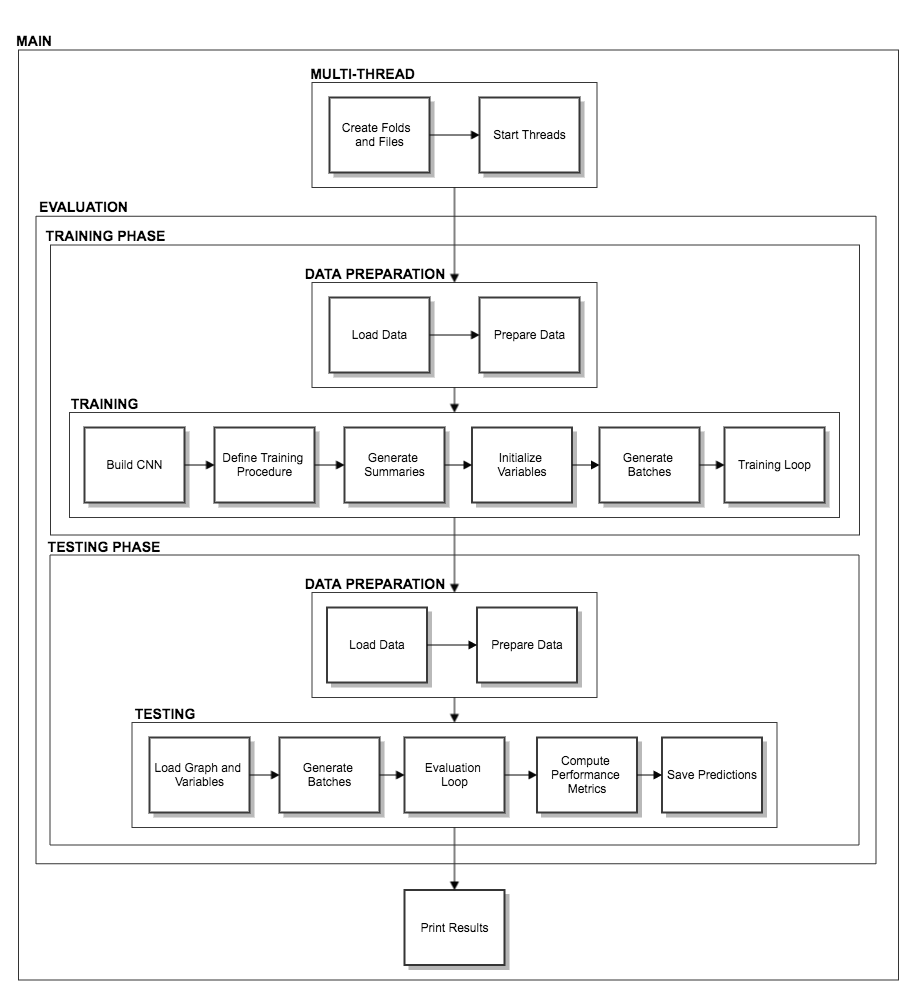
\includegraphics[width=\linewidth]{figs/CNNProcess.png}
	\caption{Process for building and applying a CNN.}
	\label{fig:CNNProcess}
	\vspace{-4mm}
\end{figure}

Figure \ref{fig:CNNProcess} provides an overview of the CNN process. To increase the training speed and to benefit as much as possible from the processing power available, several threads are created. One thread is started for each fold, using a pair of previously generated training files. Up to five threads can be processed at the same time. The next actions are all performed simultaneously on each thread, until we have models trained for all folds. 

The evaluation process consists of two main phases: the training and the testing phase. In the former, some data preparation is required: load the two training sets, build the vocabulary, shuffle, and split the dataset in a training and development set. 

\section{Study Definition}

0.5 page

\subsection{Dataset}

1.5 page

\subsection{Analysis Method}

2 pages

\section{Study Results}

\subsection{Source Code Comments Only}

1.5 pages 

% \Desktop\CNN-results.csv
% \noiseux1523\cnn-text-classification-tf-w2v 
%		dans \encoded-comment-files pour le data
%		dans \run-all.sh pour le process

\subsection{Source Code With Comments}

1.5 pages

% \Desktop\stats-baseline-with comments.csv
% dans \yes-and-no pour le data
% dans \run-all.v2.sh pour le process

design et implementation

\subsection{Source Code Without Comments}

1.5 pages

% \Desktop\stats-baseline-with-no-comments.csv
% dans \yes-and-no pour le data
% dans \run-all.v2.sh pour le process

design et implementation

\subsection{Source Code Partially With Comments}

1.5 pages

% \Desktop\stats-baseline-no-manually-tagged-comments.csv
% dans \yes-and-no pour le data
% dans \run-all.v2.sh pour le process

design et implementation


